\documentclass[12pt]{article}

\usepackage{styles/sbc-template}
\usepackage{graphicx,url}
\usepackage[utf8]{inputenc}
\usepackage[american]{babel}
% two images, same frame, side by side
\usepackage{subfig}

\sloppy

\title{Exploring Energy Flow Classifier to Identify \\ Fraudulent Cryptocurrency Transactions}

\author{Kevin S. Araujo\inst{1}, Rodrigo Bonifacio de Almeida\inst{1}, 
  Fabiano Cavalcanti Fernandes\inst{2} }


\address{Departamento de Ciências da Computação -- Universidade de Brasília (UnB) \\
  -- Campus Universitário Darcy Ribeiro, Brasília-DF
\nextinstitute
  Instituto Federal de Brasília (IFB) -- Taguating, DF -- Brazil
  \email{kevin.araujo@aluno.unb.br, rbonifacio@unb.br, fabiano.fernandes@ifb.edu.br}
}

\begin{document} 

\maketitle

\begin{abstract}
  This is a work in progress.
\end{abstract}

\section{Introduction} \label{sec:introduction}
Bitcoin is an electronic transaction system operating without a third-party moderator~\cite{nakamoto2008bitcoin}. It is built
upon blockchain technology, where an immutable ledger of financial transactions is maintained through mathematics, programming,
and advanced cryptography. This distributed ledger architecture eliminates the need for central authorities to establish trust.
Although Bitcoin was designed to circumvent vulnerabilities in the traditional financial system \cite{nakamoto2008bitcoin},
it is not immune to manipulation and anomalous activities, necessitating robust detection mechanisms~\cite{fang2022cryptocurrency,
zhang2020financial,zainal2018review}. 

Indeed, cryptocurrency-related fraud has emerged as a significant threat, causing substantial financial losses and shaking
trust in the digital asset ecosystem. In 2023, for instance, illicit addresses received \$24.2 billion in cryptocurrency,
indicating the scale of financial losses from scams, stolen funds, and other illicit activities \cite{chainalysis2024cryptocrime}.
These activities not only cause direct monetary damage to individuals and institutions but also have broader implications,
such as undermining the legitimacy of cryptocurrency markets and hindering the widespread adoption of blockchain technology.
The need to develop effective methods for detecting and preventing cryptocurrency fraud is crucial to protect participants,
maintain market integrity, and ensure the sustainable growth of the cryptocurrency industry \cite{scharfman2024, Khiari2025}.

However, detecting anomalous patterns within the intricate data streams of cryptocurrency transactions poses a significant
challenge. Like many modern datasets, these transactions are characterized by high dimensionality, evolving characteristics,
and a substantial volume, which complicates the application of traditional anomaly detection methods. In this context, the
Energy-based Flow Classifier (EFC) presents a promising approach rooted in statistical physics. Originally formulated using
the Inverse Potts model \cite{pontes2019}, the EFC characterizes the probability distribution of normal data flows through
an energy function derived from observed data patterns \cite{pontes2019}. Previous research has demonstrated the utility
of EFC in classifying unusual network traffic, suggesting its potential for adapting to detect fraudulent activity within
cryptocurrency systems \cite{pontes2019, souza2022novelopensetenergybased}.

Building upon the promise of the Energy-based Flow Classifier (EFC) framework, this paper presents a comprehensive empirical
evaluation of its application to detecting illicit Bitcoin transactions. To this end, we first replicate a previous study
that employs machine learning algorithms such as K-Nearest Neighbors, One-Class Support Vector Machine, and Isolation Forest
for anomaly detection on the Elliptic dataset \footnote{Available at https://www.kaggle.com/ellipticco/elliptic-data-set}.
We then investigate the use of EFC as a potential alternative to these machine learning approaches, using the same dataset
for consistency. Our findings confirm the EFC's ability to distinguish between licit and illicit transaction patterns based
on their energy profiles, showing strong performance in identifying illegal activity even when trained solely on licit data.
However, the results also highlight the critical sensitivity to specific configuration parameters. In particular, we observe
significant trade-offs between maximizing the detection rate of illicit transactions (recall) and minimizing false positives
(precision), especially concerning the energy threshold that defines anomalous behavior. Addressing the significant challenge
of label scarcity inherent in datasets like Elliptic is crucial for developing effective fraud detection systems.
Traditional supervised machine learning methods often struggle in such scenarios due to the limited availability of
labeled illicit examples. This motivates the exploration of alternative approaches, particularly those capable of learning
from predominantly normal data. The Energy-based Flow Classifier (EFC) emerges as a promising candidate in this regard.
Originally proposed for network intrusion detection \cite{pontes2019, souza2022novelopensetenergybased}, EFC was designed
specifically to address key limitations of conventional ML classifiers, including the reliance on extensive labeled datasets.
A core strength highlighted in its foundational work is its ability to function as an anomaly-based classifier, inferring
a statistical model of normal behavior using only labeled *benign* (or licit, in our context) examples
\cite{souza2022novelopensetenergybased}. Deviations from this learned norm, characterized by higher 'energy' scores, are
then flagged as potential anomalies. This one-class learning paradigm directly tackles the label scarcity issue prevalent
in the Elliptic dataset, allowing us to model legitimate transaction patterns effectively even with few confirmed illicit
instances. Furthermore, EFC's demonstrated adaptability across different data distributions in network traffic analysis
suggests potential robustness in the dynamic environment of cryptocurrency transactions. Consequently, this paper evaluates
the suitability and performance of EFC for identifying illicit Bitcoin transactions by leveraging its capacity to model
normality from available licit data.

In summary, the main contributions of this paper are:

\begin{itemize}
    \item Novel Application and Empirical Evaluation of EFC for One-Class Bitcoin Anomaly Detection;
    \item c2
    \item c3
\end{itemize}

\section{Background and Related Work} \label{sec:background}
Financial market manipulation, traditionally associated with actions taken by state-level entities often concerning currency
exchange rates \cite{domanski2011currency, market_manipulation_detection_2022}, takes on a different character in the realm
of cryptocurrencies. Cryptocurrency manipulation typically involves deceptive strategies employed by individuals or coordinated
groups aiming to artificially distort market prices or activity, usually for illicit profit \cite{cryptocurrency_arket_manipulation_2021}.
Understanding these tactics is crucial for developing effective detection mechanisms.

Among the prevalent forms of cryptocurrency fraud are pump-and-dump schemes and wash trading. \textbf{Pump-and-dump fraud}
involves orchestrating an artificial inflation of a cryptocurrency's price ("pump") through misleading promotions or coordinated
buying, attracting unsuspecting investors. The manipulators then sell their holdings ("dump") at the peak price, causing
a market crash and significant losses for later investors \cite{karim2018manipulation}. \textbf{Wash trading}, conversely,
creates a false impression of high trading volume and liquidity. This is achieved when an entity or colluding group
simultaneously buys and sells the same asset, often using multiple accounts or automated bots, effectively trading with
themselves. The goal is to make the asset appear more active and desirable than it is, thereby manipulating market sentiment
and potentially influencing its price \cite{gandal2018price, edelman2018detecting}. The decentralized and pseudonymous
nature of many cryptocurrency platforms can exacerbate the challenges in detecting and preventing such manipulations.

Addressing the challenge of identifying anomalous patterns within complex data streams, such as financial transactions,
requires robust methodologies. One promising approach, grounded in statistical physics, is the \textbf{Energy-based Flow Classifier (EFC)}.
Originally proposed using the Inverse Potts model to analyze network traffic data \cite{pontes2019}, EFC operates on the
principle of assigning an "energy" score to data points or flows. The model is trained to learn the probability distribution
of normal system behavior, associating typical, expected patterns (e.g., legitimate transactions) with low-energy states.
Conversely, configurations that deviate significantly from this learned normality, potentially representing anomalies or
malicious activities, manifest as high-energy states. This energy score provides a quantitative measure of typicality.
Subsequent research has extended the EFC framework, demonstrating its utility in classifying unusual network traffic for
intrusion detection and highlighting its potential for open-set recognition—identifying novel anomalies not seen during
training \cite{pontes2019, souza2022novelopensetenergybased}.

The EFC framework appears particularly well-suited for detecting anomalous Bitcoin transactions for several key reasons.
Firstly, its fundamental design as an anomaly detector allows it to learn the characteristics of *normal* (Licit) behavior,
often from unlabeled or predominantly normal data. It then identifies anomalies (potentially Illicit transactions) as
deviations exhibiting high 'energy' relative to this learned norm. This inherent capability to operate in a one-class or
unsupervised manner directly addresses the significant challenge of label scarcity common in financial fraud datasets like
Elliptic \cite{bansal2022systematic}. Secondly, the energy function provides a holistic measure derived from
the interplay of multiple features, potentially capturing complex, subtle deviations in the high-dimensional feature space
of Bitcoin transactions that simpler methods might miss \cite{wilson2024future}. Given its prior success in
analogous domains involving complex flow data \cite{pontes2019, souza2022novelopensetenergybased}, we hypothesize that
EFC's unique characteristics offer advantages for identifying illicit activities within the Bitcoin blockchain.

Detecting illicit transactions in cryptocurrencies is fundamentally an anomaly detection task. Various approaches have been 
explored, ranging from rule-based systems identifying known patterns to sophisticated machine learning techniques
\cite{samariya2023comprehensive, li2023survey}.
Traditional anomaly detection methods often face challenges when applied to cryptocurrency data due to its high dimensionality,
the dynamic and evolving nature of transaction patterns, significant class imbalance (illicit transactions being rare), and
the sheer volume of data \cite{pallathadka2022cryptocurrency}. Techniques like statistical process control, clustering-based
methods (e.g., DBSCAN, k-means variations), and distance-based methods (e.g., k-Nearest Neighbors anomaly detection)
have been applied, each with varying degrees of success and limitations, particularly concerning scalability and the ability
to capture complex, non-linear relationships \cite{hilal2022financial}.

Building on these general principles, numerous machine learning models have been specifically investigated for identifying
fraud and money laundering within the Bitcoin ecosystem. Supervised learning approaches, such as Random Forests, Support
Vector Machines (SVM), Multilayer Perceptrons (MLP), and Gradient Boosting Machines, have shown promise when sufficient
labeled data is available \cite{lorenz2021machinelearningmethodsdetect, chen2021bitcoin}. However, their performance heavily
relies on the quality and quantity of labeled examples, which is often a bottleneck. Consequently, semi-supervised and
unsupervised methods, including One-Class SVM (OC-SVM) and Isolation Forests, have gained attention as they can leverage
unlabeled data or focus solely on modeling normal behavior \cite{lorenz2021machinelearningmethodsdetect, kehinde2024machine}.
More recently, Graph Neural Networks (GNNs) have emerged as a powerful tool, explicitly leveraging the graph structure of
the blockchain to capture relational information between transactions, which can be crucial for identifying complex illicit
schemes \cite{weber2019antimoneylaunderingbitcoinexperimenting}. Our work contributes to this landscape by evaluating
EFC, an alternative physics-inspired one-class approach, assessing its performance against the backdrop of these established
techniques, particularly focusing on its behavior under label scarcity.

\section{Study Settings} \label{sec:methods}
This section details the data and methods employed in our study, which builds upon the foundational research presented
by \cite{lorenz2021machinelearningmethodsdetect}. That work explored the use of various machine learning classifiers
(e.g., Random Forest, SVM, MLP) applied to engineered features from the Elliptic dataset to identify illicit Bitcoin transactions,
specifically tackling the inherent challenge of label scarcity. While demonstrating the potential of standard ML techniques,
their approach relied on supervised or semi-supervised frameworks requiring at least some labels. Our research
diverges by investigating the Energy Flow Classifier (EFC). 

\subsection{Dataset Description} \label{subsec:dataset}
This study utilizes the Elliptic dataset, a publicly available graph dataset of Bitcoin transactions introduced by 
\cite{weber2019antimoneylaunderingbitcoinexperimenting} and subsequently used in foundational studies on machine
learning for Bitcoin money laundering detection, including the work by~\cite{lorenz2021machinelearningmethodsdetect}
which highlighted the challenges of label scarcity. The dataset represents a temporal subgraph of the public Bitcoin
blockchain, focusing on transactions involving entities identified by Elliptic Ltd., a company specializing in blockchain
analytics and financial crime prevention. It captures transaction patterns over 49 distinct time steps, where each step
corresponds roughly to a two-week period. The full dataset comprises 203,769 transaction nodes and 234,355 directed edges
representing the flow of Bitcoin between transactions.

Each transaction (node) in the graph is described by a set of 166 anonymized features. One feature explicitly denotes the
time step (1 to 49). The remaining 165 features are local transactional properties, including aggregated information about
the transaction's inputs and outputs (e.g., number, amounts, fees) and potentially aggregated statistics from its immediate
neighborhood in the transaction graph. These features are provided in a normalized or standardized form, obscuring raw
values but preserving relational patterns crucial for machine learning analysis. The graph structure itself, defined by
the edges connecting transactions where the output of one becomes the input of another, provides contextual information
about the flow of funds---although our EFC implementation primarily focuses on the
node features. A key characteristic of the Elliptic dataset is its label scarcity---while the entire dataset contains over
200,000 transactions, only a subset of 46,564 transactions is explicitly labeled. This represents a central challenge addressed by 
\cite{lorenz2021machinelearningmethodsdetect} and serves as a motivation for exploring EFC in this domain.  
The labels classify transactions into two main categories:

\begin{description}
    \item [Licit Transactions:] Transactions associated with known legitimate entities such as exchanges, miners, wallet providers,
      and other regulated services (42,019 instances in the original labeled set).
    \item [Illicit Transaction:] Transactions linked to known illicit activities, including scams, ransomware, terrorist financing,
      Ponzi schemes, and dark market operations (4,545 instances in the original labeled set).
\end{description}

\begin{table}[htbp]
  \centering
  \caption{Summary Statistics of the Elliptic Dataset (based on \cite{weber2019antimoneylaunderingbitcoinexperimenting}).}
  \label{tab:dataset_summary}
  \begin{tabular}{lr}
    Characteristic        & Value \\
    Total Transactions (Nodes) & 203,769 \\
    Total Edges           & 234,355 \\
    Time Steps            & 49 \\
    Features per Node     & 166 \\
    Labeled Transactions  & 46,564 (\textasciitilde23\%) \\
    \quad - Licit         & 42,019 (\textasciitilde90.2\% of labeled) \\
    \quad - Illicit       & 4,545 (\textasciitilde9.8\% of labeled) \\
    Unlabeled Transactions & 157,205 (\textasciitilde77\%) \\
  \end{tabular}
\end{table}

\subsection{Data Preprocessing} \label{subsec:preprocessing}
Preparing the Elliptic dataset for EFC involved several key steps focused on handling labels, selecting relevant features,
scaling the data appropriately, and partitioning it for training and evaluation in a temporally meaningful way.

To prepare the dataset (Section~\ref{subsec:dataset}), we filtered transactions based on their assigned labels. Since the
EFC model learns patterns from \textit{normal} data to detect anomalies, transactions labeled as \textit{Licit} were used
as the normal class for training. In contrast, transactions labeled as \textit{Illicit} were treated as anomalies and reserved
for evaluation. Transactions with \textit{Unknown} labels were excluded from both training and testing to ensure that the
evaluation relied solely on transactions with a known ground truth. For the binary classification task (\textit{licit} vs. \textit{illicit}),
labels were mapped to numerical values—0 for licit and 1 for illicit.

Second, we performed feature selection and transformation. Of the 166 features available for each transaction, the feature
explicitly indicating the time step (ranging from 1 to 49) was removed. While this temporal information was essential for
partitioning the data, it was excluded from the EFC model's input, as the model focuses on intrinsic transaction properties
rather than absolute temporal position. The remaining 165 anonymized features---representing transactional and local graph
characteristics---were retained as inputs to the EFC. Although the original dataset description reports some form of
normalization~\cite{weber2019antimoneylaunderingbitcoinexperimenting}, we decided to apply the Min-Max scaling to the
[0, 1] range to ensure consistency and enhance the stability of energy calculations within the EFC framework. Scaling was
applied separately to the training and test sets, with the scaler fitted exclusively on the training data to prevent data leakage.

Third, we implemented a temporal data split, in line with common practice for this dataset 
\cite{weber2019antimoneylaunderingbitcoinexperimenting, lorenz2021machinelearningmethodsdetect}, to simulate a realistic
scenario in which a model trained on historical data is used to detect fraudulent activity in future transactions.
Transactions from time steps 1 to 34 were allocated to the training set, while those from time steps 35 to 49 were reserved
for testing. The EFC model was trained exclusively on licit (normal) transactions from the training period (time steps 1-34).
The test set (time steps 35-49) included both licit and illicit transactions, enabling an evaluation of the model's ability
to assign higher energy scores to previously unseen illicit transactions compared to unseen licit ones.

\subsection{Energy Flow Classifier Configuration} \label{subsec:efc_implementation}

For detecting illicit transactions within the Elliptic dataset, we employed the Energy Flow Classifier (EFC), leveraging
the Python package implementation \cite{efc_package_github} based on the recommendations by Pontes et al.
\cite{pontes2019,souza2022novelopensetenergybased}. EFC operates on the premise that normal system behavior corresponds
to low-energy states, while anomalies or deviations manifest as high-energy states. Our implementation specifically
utilizes EFC as a one-class anomaly detector, tailored to the label scarcity challenge inherent in the dataset.

To set up EFC in our experiment, we extended the class-based interface provided by the EFC Python package, specifically
by overriding the \texttt{EnergyBasedFlowClassifier} class to tailor its behavior to our evaluation needs. In our implementation,
we configured three key EFC hyperparameters: \texttt{n\_bins}, \texttt{cutoff\_quantile}, and \texttt{pseudocounts}.
The \texttt{n\_bins} parameter controls the discretization of input features, dividing each feature's range into a specified
number of bins. These bins form the basis for estimating state probabilities and computing energy values. Based on preliminary
experiments~\cite{reproducibility}, we used \texttt{n\_bins = 30}. The \texttt{cutoff\_quantile} parameter sets the anomaly
threshold by determining the energy value corresponding to a quantile of the training data's energy distribution. For instance,
a setting of \texttt{cutoff\_quantile = 0.90} classifies any sample with an energy score above the 90th percentile as anomalous.
Finally, \texttt{pseudocounts} addresses the issue of zero probabilities when encountering states not seen in the training
data. We used a small \texttt{pseudocounts} of \texttt{0.10} to ensure numerical stability during energy computation.

Regarding the \emph{training process}, a central aspect of our EFC configuration is its alignment with the anomaly detection
setting under label scarcity. As outlined in Section~\ref{subsec:preprocessing}, the EFC model was trained exclusively on
licit (normal) transactions from the training period (time steps 1--34) by invoking its \texttt{fit} method. This follows
the one-class classification paradigm, in which the model learns the energy landscape associated with legitimate Bitcoin
transactions based solely on verified normal examples. Illicit transactions were entirely excluded from the training phase
to preserve the model's ability to generalize and detect anomalies without prior exposure to them.

During the evaluation phase, the trained EFC model's \texttt{predict} method was applied to the test set---transactions
from time steps 35--49, which contained both licit and illicit instances. For each test transaction, the EFC computed an
energy score based on its features and the probability distributions learned during training. If a transaction's energy
score exceeded the pre-determined cutoff threshold (derived from the \texttt{cutoff\_quantile} applied to the training data's
energy distribution), it was classified as anomalous (predicted illicit); otherwise, it was classified as normal (predicted licit).
The energy scores were also used to compute evaluation metrics such as AUC, which assess ranking performance rather than
relying on a fixed classification threshold.

\section{Goal, Questions, and Metrics} \label{subsec:task}
The primary goal of this study is to evaluate the effectiveness of the Energy Flow Classifier (EFC), configured
as described in Section \ref{subsec:efc_implementation}, for identifying illicit transactions within the Elliptic
Bitcoin dataset. This aligns with the broader goal of exploring alternative methodologies, particularly those suited for
label scarcity, compared to the supervised approaches examined by \cite{lorenz2021machinelearningmethodsdetect}. Our aim
is to answer the following research question: \emph{How effective is the Energy-Based Flow Classifier (EFC) under conditions
of label scarcity in identifying illicit transactions in the Elliptic Bitcoin dataset?}

Specifically, our research is thus framed as a \emph{one-class anomaly detection problem}. Having trained the EFC model exclusively
on Licit transactions from the initial time steps (1-34), the objective is to assess its ability to distinguish between
licit and illicit transactions in the subsequent, unseen time steps (35-49) of the test set. This evaluation involves
two main perspectives:

\begin{enumerate}
    \item \textbf{Classification Performance:} Using the energy threshold derived from the training data, based on the
      \texttt{cutoff\_quantile}, we assess how well EFC classifies unseen transactions as either licit (below threshold)
      or illicit (above threshold). Performance is measured using standard classification metrics suitable for imbalanced
      datasets, such as Precision, Recall, F1-Score, and potentially Balanced Accuracy, calculated on the labeled test set.
      
    \item \textbf{Ranking Performance:} Independent of a specific threshold, we evaluate EFC's ability to assign consistently
      higher energy scores to illicit transactions compared to licit transactions in the test set. This is primarily
      assessed using the Area Under the Receiver Operating Characteristic Curve (AUC-ROC), which measures the model's
      ability to rank anomalies higher than normal instances across all possible thresholds.
\end{enumerate}

The outcome of this research may provide insights into the potential of EFC as a viable tool for detecting fraudulent or
anomalous Bitcoin transactions. By leveraging its unsupervised, energy-based approach, EFC aims to address challenges such
as label scarcity and to identify novel deviations from normal transaction behavior.

\section{Results} \label{sec:results}
This section presents the empirical findings from the application of the Energy Flow Classifier (EFC) to the task of
identifying illicit transactions within the Elliptic Bitcoin dataset. Following the methodology outlined in Section
\ref{sec:methods}, the EFC was employed primarily as a one-class anomaly detector, trained exclusively on transactions
labeled as Licit from the initial time steps (1-34). The core objective was to evaluate the model's capability to distinguish
these known Licit patterns from potentially anomalous Illicit transactions present in the unseen test set (time steps 35-49).
Performance is assessed based on the EFC's ability to assign distinct energy scores to the two classes and evaluated using
metrics appropriate for imbalanced anomaly detection scenarios. The subsequent subsections detail the outcomes of specific
experiments conducted, focusing on the model's baseline performance and sensitivity to key configuration parameters under
the defined experimental setup.

\subsection{Shared Experimental Setup} \label{subsec:shared_setup}
Unless explicitly stated otherwise in the description of a specific experiment, the following setup, derived from the procedures
detailed in Section \ref{sec:methods}, was consistently used across the results presented below:

\begin{itemize}
    \item \textbf{Dataset Split:} The EFC model was trained exclusively on transactions labeled as Licit from time steps
      1 to 34. Evaluation was performed on the test set containing both Licit and Illicit transactions from time steps
      35 to 49. Transactions labeled 'Unknown' were excluded from both training and testing.
    \item \textbf{Feature Set:} The input to the EFC model consisted of the 165 anonymized features described in Section
      \ref{subsec:dataset}, after removing the time step feature. These features were scaled to the range [0, 1] using
      Min-Max scaling, with the scaler fitted only on the training data (Licit transactions, steps 1-34).
    \item \textbf{EFC Configuration:} The core EFC implementation (Section \ref{subsec:efc_implementation}) utilized the
      following default hyperparameters based on initial tuning and common practice:
        \begin{itemize}
            \item Number of bins for feature discretization \texttt{n\_bins=30}
            \item Cutoff quantile for anomaly threshold \texttt{cutoff\_quantile=0.9} (meaning the energy threshold is set at
              the 90th percentile of the energy distribution of the Licit training data)
            \item Pseudocounts \texttt{pseudocounts=0.1} (to handle zero probabilities)
        \end{itemize}
        \item \textbf{Evaluation Metrics \& Outputs:} Model performance was assessed using a combination of quantitative
          metrics and qualitative analysis:
          \begin{itemize}
              \item \textbf{F1-Score (Macro Average):} As the primary evaluation metric, we adopted the macro-averaged F1-score,
                consistent with the benchmark study by \cite{lorenz2021machinelearningmethodsdetect}. This metric calculates the
                F1-score for each class (Licit and Illicit) independently and then averages them, providing a balanced measure
                of performance across both classes, which is crucial given the inherent class imbalance.
              \item \textbf{Class-Specific Metrics (Illicit Class):} While F1-Macro provides an overall view, our primary
                interest lies in detecting the Illicit class (class 1). Therefore, we also report Precision, Recall, and
                the F1-Score specifically calculated for the Illicit class based on the classification derived from the
                \texttt{cutoff\_quantile} threshold. These metrics offer direct insight into the model's effectiveness in
                identifying illicit transactions and the associated trade-offs (e.g., false positives vs. false negatives).
              \item \textbf{EFC Energy Distributions:} For each experiment, histograms comparing the distribution of EFC
                energy scores assigned to Licit versus Illicit transactions in the test set were generated. These plots
                  provide a visual assessment of the model's separation capability.
              \item \textbf{Detailed Results Storage:} Key information for each experimental run, including the sizes of
                the training and testing datasets (and their class distributions), the calculated performance metrics,
                and the confusion matrix, were systematically collected and saved into individual CSV files for detailed
                comparison and analysis across experiments.
          \end{itemize}
\end{itemize}

The following subsections will now present the results from the specific experiments conducted under this framework, highlighting
deviations from this shared setup where applicable.

\subsection{Experiments} \label{subsec:experiments}

This section details the experimental evaluations conducted to assess the proposed methodologies. We performed three primary
experiments focusing on data balancing, feature engineering/selection, and model comparison/tuning, respectively. All
experiments utilized the EFC dataset, preprocessed as described previously, employing a standard train-test split methodology.

\subsection{Experiment 1: Impact of Data Balancing Techniques} \label{subsec:experiment_1}
This experiment investigated the effect of various data balancing strategies on classification performance for the inherently
imbalanced EFC dataset. The baseline performance was established using the original, unbalanced dataset. This was compared
against four common balancing techniques applied to the training dataset and test dataset: creating a balanced subset with
equally distributed classes, by undersampling the majority class before splitting, Synthetic Minority Over-sampling Technique
(SMOTE), Random Oversampling of the minority class, and Random Undersampling of the majority class. The test set composition
remained consistent across most techniques to ensure fair evaluation. Performance was evaluated using Accuracy, Precision,
Recall, F1-Score (weighted), Macro F1-Score, and confusion matrices. Table~\ref{tab:efc_consolidated_results} summarizes
the dataset characteristics after applying each technique and the corresponding classification results.

\begin{figure}[!tph]
  \centering
  \subfloat[Unbalanced Dataset.]{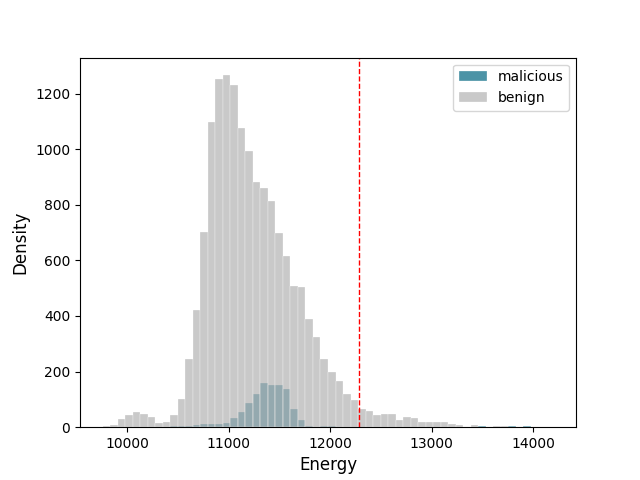
\includegraphics[width=0.4\textwidth]{figures/experiment-1/1_unbalanced_dataset.png}\label{fig1:1_unbalanced_dataset}}
  \subfloat[Balanced Dataset.]{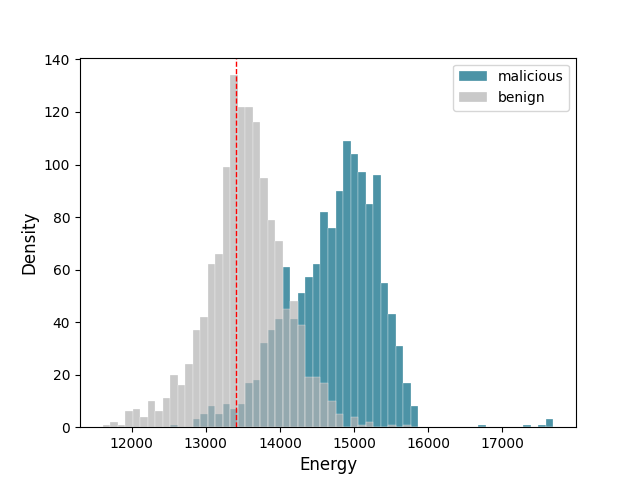
\includegraphics[width=0.4\textwidth]{figures/experiment-1/2_balaced_dataset.png}\label{fig2:2_balaced_dataset}}
  \subfloat[SMOTE.]{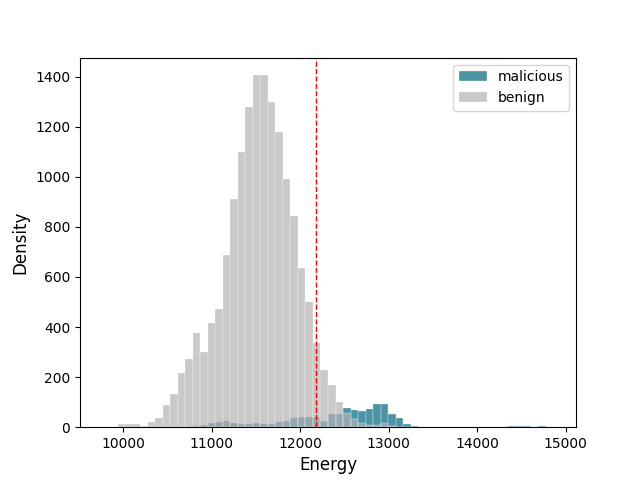
\includegraphics[width=0.4\textwidth]{figures/experiment-1/3_smote_minority_full_test_dataset.png}\label{fig3:3_smote_minority}}
  \caption{Experiment 1: Energy Distribution Of Licit and Illicit Transactions.}
\end{figure}

\subsection{Experiment 2: Impact of Feature Selection} \label{subsec:experiment_2}
Following the analysis of data balancing, Experiment 4 focused on evaluating 
the impact of feature selection on classification performance using the Energy-Based Flow Classifier (EFC). We employed
the \texttt{SelectKBest} algorithm from scikit-learn, utilizing the ANOVA F-value (\texttt{f\_classif}) scoring function
to rank and select features based on their relevance to the class labels. The experiment systematically varied the number
of selected features, testing values of $k \in {10, 20, 30, 40, 50, 60}$. The feature selection process using \texttt{SelectKBest}
was applied to the features and labels of the original unbalanced dataset \textit{before} the standard train-test split
was performed on the resulting reduced feature set. Furthermore, we conducted two distinct series of runs: one applying
feature selection to the complete feature set, including aggregated temporal features, and another applying it only to
the raw node features after explicitly excluding the aggregated ones. The decision to conduct feature selection in two
distinct scenarios within Experiment 2---one including the aggregated neighborhood statistics and one explicitly excluding
them---was driven by the need to understand the specific impact and contribution of these aggregated features. Aggregated
features, which represent statistical summaries of a node's neighborhood (as described in related financial forensics
work, e.g., \cite{weber2019antimoneylaunderingbitcoinexperimenting}), often possess high individual predictive power due
to the condensed information they carry about local graph structure. Including these potentially dominant features in the
\texttt{SelectKBest} process (Scenario 1) could lead to them consistently ranking highest, potentially masking the predictive
contribution of the node's intrinsic, raw features. By running a separate scenario (Scenario 2) where these aggregated
features were removed \textit{before} applying \texttt{SelectKBest}, we aimed to isolate and evaluate the predictive
capability derived solely from the raw node characteristics. This allows for a clearer comparison and a better understanding
of which feature types (raw vs. aggregated) are most crucial for classification, especially when operating under the
dimensionality constraints imposed by selecting only the top $k$ features.

Performance for each value of $k$ and for both feature set scenarios (with and without aggregated features) was assessed
using the same metrics as Experiment 3 (Accuracy, Precision, Recall, F1-Score, Macro F1-Score). The objective was to
determine if reducing dimensionality could maintain or improve performance, identify an optimal number of features ($k$),
and understand the contribution of aggregated features within this selection context.

\begin{figure}[!tp]
  \centering
  \subfloat[k=10.]{\includegraphics[width=0.30\textwidth]{figures/experiment-2/1-Feature Selection Excluding Aggregate Features,
  Increasing Value of k={k_size}/Feature Selection Excluding Aggregate Features, Increasing Value of k=10.png}\label{fig4:fs_no_agg_k_10}}
  \hfill

  \subfloat[k=20.]{\includegraphics[width=0.30\textwidth]{figures/experiment-2/1-Feature Selection Excluding Aggregate Features,
  Increasing Value of k={k_size}/Feature Selection Excluding Aggregate Features, Increasing Value of k=20.png}\label{fig5:fs_no_agg_k_20}}
  \hfill

  \subfloat[k=30.]{\includegraphics[width=0.30\textwidth]{figures/experiment-2/1-Feature Selection Excluding Aggregate Features,
  Increasing Value of k={k_size}/Feature Selection Excluding Aggregate Features, Increasing Value of k=30.png}\label{fig6:fs_no_agg_k_30}}
  \hfill

  \subfloat[k=40.]{\includegraphics[width=0.30\textwidth]{figures/experiment-2/1-Feature Selection Excluding Aggregate Features,
  Increasing Value of k={k_size}/Feature Selection Excluding Aggregate Features, Increasing Value of k=40.png}\label{fig7:fs_no_agg_k_40}}
  \hfill

  \subfloat[k=50.]{\includegraphics[width=0.30\textwidth]{figures/experiment-2/1-Feature Selection Excluding Aggregate Features,
  Increasing Value of k={k_size}/Feature Selection Excluding Aggregate Features, Increasing Value of k=50.png}\label{fig8:fs_no_agg_k_50}}
  \hfill

  \subfloat[k=60.]{\includegraphics[width=0.30\textwidth]{figures/experiment-2/1-Feature Selection Excluding Aggregate Features,
  Increasing Value of k={k_size}/Feature Selection Excluding Aggregate Features, Increasing Value of k=60.png}\label{fig9:fs_no_agg_k_60}}

  \caption{Experiment 2, Technique A: Feature Selection Excluding Aggregate Features, Increasing Value of k, Energy
  Distribution Of Licit and Illicit Transactions.}

\end{figure}

\begin{figure}[!tbp]
  \centering
  \subfloat[k=10.]{\includegraphics[width=0.30\textwidth]{figures/experiment-2/2-Feature Selection Excluding Aggregate Features,
  Increasing Value of k={k_size}/Feature Selection, Increasing Value of k=10.png}\label{fig10:fs_agg_k_10}}
  \hfill

  \subfloat[k=20.]{\includegraphics[width=0.30\textwidth]{figures/experiment-2/2-Feature Selection Excluding Aggregate Features,
  Increasing Value of k={k_size}/Feature Selection, Increasing Value of k=20.png}\label{fig11:fs_agg_k_20}}
  \hfill

  \subfloat[k=30.]{\includegraphics[width=0.30\textwidth]{figures/experiment-2/2-Feature Selection Excluding Aggregate Features,
  Increasing Value of k={k_size}/Feature Selection, Increasing Value of k=30.png}\label{fig12:fs_agg_k_30}}
  \hfill

  \subfloat[k=40.]{\includegraphics[width=0.30\textwidth]{figures/experiment-2/2-Feature Selection Excluding Aggregate Features,
  Increasing Value of k={k_size}/Feature Selection, Increasing Value of k=40.png}\label{fig13:fs_agg_k_40}}
  \hfill

  \subfloat[k=50.]{\includegraphics[width=0.30\textwidth]{figures/experiment-2/2-Feature Selection Excluding Aggregate Features,
  Increasing Value of k={k_size}/Feature Selection, Increasing Value of k=50.png}\label{fig14:fs_agg_k_50}}
  \hfill

  \subfloat[k=60.]{\includegraphics[width=0.30\textwidth]{figures/experiment-2/2-Feature Selection Excluding Aggregate Features,
  Increasing Value of k={k_size}/Feature Selection, Increasing Value of k=60.png}\label{fig15:fs_agg_k_60}}
  \hfill
    
  \caption{Experiment 2, Technique B: Feature Selection Including Aggregate Features, Increasing Value of k, Energy
  Distribution Of Licit and Illicit Transactions.}

\end{figure}

\subsection{Experiment 3: Combining Feature Selection and Data Balancing} \label{subsec:experiment_3}
of feature selection and data balancing on the performance of the EFC classifier, building upon the findings from
Experiment 1 (data balancing) and Experiment 24 (feature selection). The core idea was to first reduce the dimensionality
of the dataset using the feature selection technique identified in Experiment 4, and then apply the SMOTE balancing
technique from Experiment 1 to the reduced-feature training data before training the EFC model.

Specifically, for each value of $k \in \{10, 20, 30, 40, 50, 60\}$, we first applied the \texttt{SelectKBest} algorithm
with the \texttt{f\_classif} scoring function to the original, unbalanced dataset (as performed in the first scenario of
Experiment 2) to obtain a dataset containing only the top $k$ features. Subsequently, this $k$-feature dataset underwent
the SMOTE procedure: it was split into training and testing sets, SMOTE was applied \textit{only} to the training portion
to balance the classes, and the EFC classifier was then trained on this balanced, feature-selected training data. Finally,
the trained EFC model was evaluated on the corresponding unbalanced test set (containing the same $k$ selected features).
Performance was assessed using the standard suite of metrics (Accuracy, Precision, Recall, F1-Score, Macro F1-Score) to
determine if applying dimensionality reduction prior to SMOTE balancing could yield improved classification performance
compared to using SMOTE on the full feature set (Experiment 1) or using feature selection alone (Experiment 2).

% \begin{figure}[!tbp]
%   \centering
%   \subfloat[k=10.]{\includegraphics[width=0.30\textwidth]{figures/experiment-3/1-SMOTE With Feature Selection, Increasing
%     Value of k={k_size}/SMOTE With Feature Selection, Increasing Value of k=10.png}\label{fig16:fs_smote_k_10}}

%   \subfloat[k=20.]{\includegraphics[width=0.30\textwidth]{figures/experiment-3/1-SMOTE With Feature Selection, Increasing
%   Value of k={k_size}/SMOTE With Feature Selection, Increasing Value of k=20.png}\label{fig17:fs_smote_k_20}}

%   \subfloat[k=30.]{\includegraphics[width=0.30\textwidth]{figures/experiment-3/1-SMOTE With Feature Selection, Increasing
%   Value of k={k_size}/SMOTE With Feature Selection, Increasing Value of k=30.png}\label{fig18:fs_smote_k_30}}

%   \subfloat[k=40.]{\includegraphics[width=0.30\textwidth]{figures/experiment-3/1-SMOTE With Feature Selection, Increasing
%     Value of k={k_size}/SMOTE With Feature Selection, Increasing Value of k=40.png}\label{fig19:fs_smote_k_40}}

%   \subfloat[k=50.]{\includegraphics[width=0.30\textwidth]{figures/experiment-3/1-SMOTE With Feature Selection, Increasing
%   Value of k={k_size}/SMOTE With Feature Selection, Increasing Value of k=50.png}\label{fig20:fs_smote_k_50}}

%   \subfloat[k=60.]{\includegraphics[width=0.30\textwidth]{figures/experiment-3/1-SMOTE With Feature Selection, Increasing
%   Value of k={k_size}/SMOTE With Feature Selection, Increasing Value of k=60.png}\label{fig21:fs_smote_k_60}}
  
%     \caption{Experiment 3, Technique A: SMOTE With Feature Selection, Increasing Value of k, Energy Distribution Of Licit
%       and Illicit Transactions.}
  
%     \caption{Experiment 3, Technique A: SMOTE With Feature Selection, Increasing Value of k, Energy Distribution Of Licit
%       and Illicit Transactions.}
% \end{figure}

% \begin{figure}[!p]
%   \centering
%   \subfloat[k=10.]{\includegraphics[width=0.30\textwidth]{figures/experiment-3/2-SMOTE With Feature Selection, Increasing
%     Value of k={k_size} Full Test Dataset/SMOTE With Feature Selection, Increasing Value of k=10 Full Test Dataset.png}
%     \label{fig22:fs_smote_full_k_10}}

%   \subfloat[k=20.]{\includegraphics[width=0.30\textwidth]{figures/experiment-3/2-SMOTE With Feature Selection, Increasing
%   Value of k={k_size} Full Test Dataset/SMOTE With Feature Selection, Increasing Value of k=20 Full Test Dataset.png}
%   \label{fig23:fs_smote_full_k_10}}

%   \subfloat[k=30.]{\includegraphics[width=0.30\textwidth]{figures/experiment-3/2-SMOTE With Feature Selection, Increasing
%   Value of k={k_size} Full Test Dataset/SMOTE With Feature Selection, Increasing Value of k=30 Full Test Dataset.png}
%   \label{fig24:fs_smote_full_k_10}}

%   \centering
%   \subfloat[k=40.]{\includegraphics[width=0.30\textwidth]{figures/experiment-3/2-SMOTE With Feature Selection, Increasing
%     Value of k={k_size} Full Test Dataset/SMOTE With Feature Selection, Increasing Value of k=40 Full Test Dataset.png}
%     \label{fig25:fs_smote_full_k_10}}
%     \hfill

%   \subfloat[k=50.]{\includegraphics[width=0.30\textwidth]{figures/experiment-3/2-SMOTE With Feature Selection, Increasing
%   Value of k={k_size} Full Test Dataset/SMOTE With Feature Selection, Increasing Value of k=50 Full Test Dataset.png}
%   \label{fig26:fs_smote_full_k_10}}
%   \hfill

%   \subfloat[k=60.]{\includegraphics[width=0.30\textwidth]{figures/experiment-3/2-SMOTE With Feature Selection, Increasing
%   Value of k={k_size} Full Test Dataset/SMOTE With Feature Selection, Increasing Value of k=60 Full Test Dataset.png}
%   \label{fig27:fs_smote_full_k_10}}
  
%   \caption{Experiment 3, Technique B: SMOTE With Feature Selection, Increasing Value of k Full Test Dataset, Energy Distribution Of Licit
%   and Illicit Transactions.}
  
%     \caption{Experiment 3, Technique B: SMOTE With Feature Selection, Increasing Value of k Full Test Dataset, Energy Distribution Of Licit
%       and Illicit Transactions.}
% \end{figure}


\begin{table*}[htbp] % table* for full page width
  \centering
  \caption{EFC Performance Summary Across Experiments: Baseline vs. Best Results from Data Balancing, Feature Selection, and Combined Approaches (Selected by F1-Macro).}
  \label{tab:efc_consolidated_results}
  \resizebox{\textwidth}{!}{
  \begin{tabular}{lrrrrrrrrr}
    \hline
    \textbf{Experiment / Technique} & \textbf{TP} & \textbf{FN} & \textbf{FP} & \textbf{TN} & \textbf{Accuracy} & \textbf{Precision} & \textbf{Recall} & \textbf{F1-Score} & \textbf{F1-Macro} \\
    & & & & & & & & \textbf{(Weighted)} & \\
    \hline
    \textbf{Exp 1: Baseline} & & & & & & & & & \\
    Unbalanced Dataset & 15117 & 470 & 1064 & 19 & 0.908 & 0.876 & 0.908 & 0.891 & 0.488 \\
    \hline
    \textbf{Exp 1: Balancing} & & & & & & & & & \\
    Best Technique (SMOTE) & 14750 & 837 & 338 & 745 & 0.929 & 0.944 & 0.929 & 0.935 & \textbf{0.760397} \\
    \hline
    \textbf{Exp 2: Feature Selection} & & & & & & & & & \\
    Best FS (Agg. Excluded, k=10) & 11317 & 598 & 598 & 766 & 0.865 & 0.893 & 0.865 & 0.877 & \textbf{0.686} \\
    Best FS (Agg. Included, k=10) & 11254 & 1352 & 560 & 804 & 0.863 & 0.895 & 0.863 & 0.876 & \textbf{0.689} \\
    \hline
    \textbf{Exp 3: FS + Balancing} & & & & & & & & & \\
    Best FS + SMOTE (k=10) & 11322 & 1284 & 368 & 996 & 0.891 & 0.931 & 0.891 & 0.891 & \textbf{0.770} \\
    \hline
  \end{tabular}
  }
  \par\medskip
  \footnotesize
  \textit{Note: TP=True Positives, FN=False Negatives, FP=False Positives, TN=True Negatives reported for the test set.
    For experiments with multiple sub-runs (varying k or balancing method), the row represents the technique yielding the
    highest F1-Macro score (shown in bold). Metrics are rounded to three decimal places. F1-Score refers to the weighted
    average unless otherwise specified.}
\end{table*}

\section{Conclusion} \label{section:conclusion}

This study evaluated the Energy Flow Classifier (EFC) as a one-class anomaly detection method for identifying illicit Bitcoin
transactions within the Elliptic dataset, focusing on scenarios with label scarcity. In evaluating the performance of the
different techniques across our experiments, we adopted the \textbf{F1-macro score} as the primary overall metric. This
choice aligns with the methodology presented by \cite{lorenz2021machinelearningmethodsdetect} in their work
on detecting money laundering in Bitcoin, particularly relevant given the common challenge of label scarcity in such datasets.
The F1-macro score is calculated by first determining the F1 score (the harmonic mean of precision and recall) for each
individual class (e.g., 'licit' and 'illicit' transactions). Then, the unweighted average of these per-class F1 scores is
taken. This approach ensures that each class contributes equally to the final metric, regardless of its frequency in the
dataset, providing a balanced assessment of model performance, especially crucial in imbalanced scenarios like fraud detection
where correctly identifying the minority class is often of high importance.

The primary advantage of EFC lies in its one-class nature, making it suitable for real-world scenarios where illicit
transaction labels are rare. However, our baseline experiment (Exp 1 - Unbalanced), using default parameters and training
only on Licit data, revealed a significant disadvantage: high sensitivity to class imbalance. While achieving high overall
accuracy (0.908) and weighted F1-score (0.891), the model performed poorly in distinguishing the minority Illicit class,
resulting in a low F1-Macro score of 0.488.

Crucially, Experiment 1 demonstrated that EFC's performance can be substantially improved through standard data preprocessing
techniques. Applying SMOTE balancing to the training data yielded the best results among the balancing methods tested,
dramatically increasing the F1-Macro score to 0.760, indicating a much more balanced detection capability across both
Licit and Illicit classes.

Further experiments explored feature selection (Exp 2) and its combination with balancing (Exp 3). Feature selection using
\texttt{SelectKBest} showed that EFC can operate with reduced dimensionality; for instance, using only the top 10 non-aggregated
features yielded an F1-Macro of 0.686, outperforming the baseline but not reaching the levels achieved with SMOTE on the full
feature set. The results for feature selection including aggregated features and the combined feature selection with SMOTE
approach (currently placeholders in Table \ref{tab:efc_consolidated_results}) require further analysis to draw definitive
conclusions about their potential benefits.

In summary, EFC presents a promising tool for detecting anomalous Bitcoin transactions, especially given its one-class
training capability. Its main drawback is a pronounced sensitivity to class imbalance, which necessitates mitigation strategies
like SMOTE balancing for effective performance (achieving F1-Macro 0.760). While feature selection is possible, careful
consideration of trade-offs is required, as dimensionality reduction might impact performance compared to using balanced,
full-feature data. The effectiveness of EFC in this context is therefore contingent on appropriate data preprocessing and
potentially hyperparameter tuning, sensitivity to which was noted in Section \ref{sec:introduction} and implied by the
experimental variations, to balance the detection of illicit activities against false alarms.


\section{Future Work} \label{sec:future_work}

While this study demonstrated the viability of the Energy Flow Classifier (EFC) for one-class anomaly detection in Bitcoin
transactions, particularly when combined with techniques like SMOTE, several open questions and avenues for future research emerge:

\begin{itemize}
    \item \textbf{Systematic Hyperparameter Optimization:} The current work used fixed default parameters (\texttt{n\_bins=30},
    \texttt{cutoff\_quantile=0.9}). An open question is how sensitive EFC's performance, especially the precision-recall
    trade-off for the Illicit class, is to these parameters.

    \item \textbf{Advanced Balancing and Cost-Sensitive Learning:} SMOTE proved effective (Exp 1), but its interaction with
    EFC's energy calculation warrants further investigation. Are there other balancing techniques (e.g., ADASYN, Tomek Links,
    Edited Nearest Neighbours) or cost-sensitive learning approaches (adjusting the EFC threshold based on misclassification
    costs) that could yield better or more robust performance, perhaps with fewer synthetic samples or different biases?

    \item \textbf{Exploring Feature Selection Synergies:} Experiments 2 and 3 explored feature selection, showing potential
    but requiring further analysis \ref{tab:efc_consolidated_results}. Key questions remain: What
    is the optimal number of features ($k$) when including aggregated features? Does the combination of FS and SMOTE truly
    outperform SMOTE alone with full features, considering both performance and computational cost?

    \item \textbf{Integration of Graph Structure:} The current EFC implementation primarily leverages node features,
    largely ignoring the rich topological information in the Elliptic graph dataset. Can explicitly incorporating transaction
    linkage improve detection?

    \item \textbf{Scalability Analysis:} How does the computational cost (training time, memory usage, prediction latency)
    of EFC scale with the number of transactions and features, especially compared to other methods?
\end{itemize}

Addressing these questions would further solidify the understanding of EFC's strengths and weaknesses in the financial
forensics domain and guide its potential practical application.


\section{Reproducibility} \label{sec:reproducibility}
To ensure the reproducibility of our findings, all code, configuration files, and scripts used for the experiments described
in this paper are made publicly available in a dedicated repository: \textbf{https://github.com/kevinsantana/PPCA-UnB-Dissertation}.

\subsection{Computational Environment} \label{subsection:environment}
The experiments were conducted on a system with the following specifications:
\begin{itemize}
    \item \textbf{Operating System:} macOS 14.5 23F79 arm64
    \item \textbf{Processor:} Apple M1 Pro
    \item \textbf{GPU:} Apple M1 Pro
    \item \textbf{Memory (RAM):} 32 GB
\end{itemize}

\bibliographystyle{sbc}
\bibliography{bibliography/sbc-template.bib}

\end{document}
